\documentclass[]{coda-art}

\graphicspath{ {./images/} {./images/logo/} }

\pretitle{Ogród Księżycowych Kwiatków\vspace*{-0.5ex}}
\title{Dotknięci Miłością}
\author{\textbf{\emph{violacoda}}, dla \textbf{\emph{Moonflowers Collective}}}

\titlecenter{%
    \vspace{1ex}
    \begin{verse}[0.7\linewidth]
        \emph{%
        \flagverse{\textcolor[HTML]{0466c8}{I:}}
        Nie pamiętam kiedy ostatni raz pozwoliłam sobie odpocząć \\
        \vin Gdy obrasta mnie księżycowych kwiatów pnącze \\
        Żyję hermetycznie, pochłonięta przez chorobliwość \\ 
        \vin Przez pryzmat której widzę i co na moich oczach rośnie}

        \vspace*{-0.25ex}\emph{%
        \flagverse{\textcolor[HTML]{9e2a2b}{E:}}
        Jesteśmy jednością rozbitą w binarność \\ 
        \vin Ja nie więcej jak gościem w Twojej domenie \\
        \vin I śmiercią zniekształconą przez Twoją projekcję \\
        Dotknięta nieśmiertelnością, aż zakwitniesz \\
        \vin Dopókiśmy rozbici nie doświadczymy śmierci \\
        \vin W inkluzji, ślepi na Miłość z której się zrodziliśmy \\
        Spętani kwiatami ogrodu chorobliwości \\ 
        \vin Pod nocną kompozycją zakwitnijmy tańcząc \\
        \vin Do samozniszczenia nas obu, by znów stać się jednym}
    \end{verse}
    \hfill {\footnotesize -- „Kwiaty Ogrodu Chorobliwości”, violacoda}
}

\titleleft{\small
    Dokument udostępniono na licencji \href{https://creativecommons.org/licenses/by/4.0/deed.pl}
    {(CC BY 4.0) \\ Creative Commons: Uznanie autorstwa}. \\[1.85ex]
%
    Jesteśmy \emph{Moonflowers Collective}, społeczność artystycznych duszyczek kwitnących pięknie nocą, jak księżycowe kwiatki.
    \emph{Ipomoea alba}, te kwiaty są dla nas symbolem dualizmu Miłości i Chorobliwości. 
    W chorobliwej nocy i cierpieniu odnajdują Miłość, światło i uzdrowienie, aby zakwitnąć prawdziwym i unikatowym pięknem. \\[1.85ex]
%
    Współtworzymy kolektyw rannych uzdrowicieli.
    Miłość jest tym, co pozwala uzdrawiać. 
    Nauczamy więc jak cierpieć świadomie i jak siebie uzdrowić sztuką Miłości.
    Wierzymy, że filozofia, psychologia, sztuka oraz Miłość, tworzą najgłębszy dialog do zrozumienia ludzkiego istnienia. \\[1.85ex]
%
    Praktykujemy postawę i filozofię, gdzie nazywamy siebie \emph{Dotkniętymi} (cierpieniem), więc \emph{Dotkniętymi Miłością}. 
    Aby nauczyć siebie i innych kochać oraz aby dotknąć ludzkie serca sztuką Miłości.
}

\noticeversion{1 maja 2023}{\emph{Wersja 0.1 alpha\hspace*{-0.3ex} 23m05a}}{%
    \vspace*{-0.5ex}
    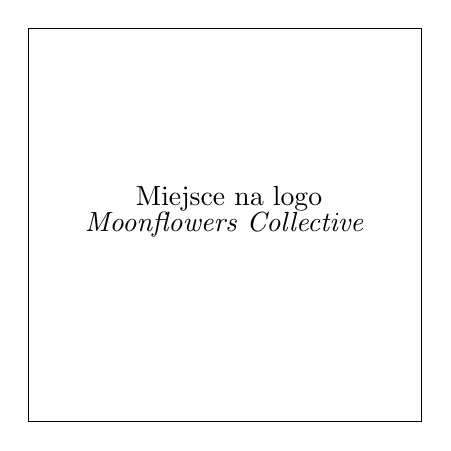
\begin{tikzpicture}
        \draw[draw=black] (0,0) rectangle (5,5)
        node[pos=.5] {\emph{Moonflowers Collective}}
        node[pos=.51,anchor=south] {Miejsce na logo};
    \end{tikzpicture} \\[0.5ex]
    \begin{flushleft}
        \hspace{2em} <moonflowers.pl wkrótce!> \\ % \href{https://moonflowers.pl}{moonflowers.pl} \\
        \hspace{2em} \img{discord} \href{https://discord.com/invite/NFRSUEztRW}{Księżycowe Kwiatki} \\
        \hspace{2em} \img{github} \href{https://github.com/violacoda/dotknieci-miloscia}{violacoda/dotknieci-miloscia}
    \end{flushleft}

}
\abstract{%
    Filozofia jest sposobem bycia, aktem życia, czyni sie ją w każdym momencie.
    Współczesna filozofia zapomniała o tej tradycji, a filozoficzny dyskurs wyprzedził filozofię jako postawę w życiu.
    Prawdziwa filozofia nie jest zlepkiem technicznego żargonu dla specjalistów, jest postawą istnienia w świecie, w ktorym praktykuje sie Miłość w każdej chwili. 
    Jej celem jest przekształcenie całego życia jednostki, aby stać się najlepszą wersją siebie.
    Prawdziwa mądrość nie sprawia, że coś po prostu wiemy: sprawia, że „jesteśmy” w inny sposób.
    Jesteśmy rannymi uzdrowicielami, Dotknięci Miłością.

    Archetyp rannego uzdrowiciela leży na dnie każdej szczerej formy uzdrawiania.
    Jej fundamentem jest budowanie głębokiej świadomości i zrozumienia własnego Ja oraz świata, w którym żyjemy.
    Dopóki czujemy się prześladowani, zgorzkniali i żywimy urazę do naszej rany, i staramy się uciec od cierpienia, pozostajemy nieuchronnie z nią związani.
    Rana może Cię zniszczyć, albo obudzić.
    Uzdrowienie swego Ja jest sprawą indywidualną, która musi wypływać z psychiki, aby istniało rozwiązanie problemu, czym jest dokładnie co termin indywiduacji implikuje.
    Sztuka Miłości to przyjęcie własnej wizji i swojego istnienia za najwyższą formę Miłości i indywidualnej ekspresji.
    To wymaga, aby spróbować pokochać chorobliwość i odważyć się rozszerzyć własną wizję, świadomie ją urzeczywistnić.
    Kochać jest trudne i brutalne.
    W chwili największej słabości, kochać to najtrudniejsze co można zrobić.
    Właśnie tego, jak kochać, ma ten dokument nauczyć.
}

\begin{document}

\maketitle

\subsection*{Struktura Dokumentu}
\emph{Akt} jest zbiorem niezależnych \emph{rozdziałów} podzielonych na \emph{części}, w których mogą znaleźć się \emph{medytacje} wyrażające przemyślane myśli na daną część rozprawy.
Dokument został podzielony na siedem aktów rozwijanych niezależnie od siebie:

\paragraph*{Akt I: Sztuka Miłości}\, --\, Fundament filozofii Dotkniętych Miłością, świadomość, istota cierpienia oraz praktyka Sztuki Miłości.

\paragraph*{Akt II: Rozwój Osobisty}\, --\, Rozprawy z intencją niesienia pomocy w indywidualnym rozwoju i rozwiązywaniu osobistych problemów.

\paragraph*{Akt III: Komunikacja i Relacje}\, --\, Zasady zdrowej komunikacji, zależności tożsamości i ego, oraz budowanie i utrzymywanie relacji międzyludzkich.

\paragraph*{Akt IV: Filozofia i Psychologia}\, --\, Przedstawienie oraz zinterpretowanie dzieł sztuki, teorii i praktyk filozoficznych oraz psychologicznych.

\paragraph*{Akt V: Natura i Nauka}\, --\, Zjawiska świata fizycznego w obserwacji i eksperymentacji, więc nauka oraz obcowanie z przyrodą.

\paragraph*{Akt VI: Ogród Księżycowych Kwiatków}\, --\, Dzieje i najważniejsze osobowości Moonflowers Collective, interpretacje i historia projektów społeczności.

\paragraph*{Akt VII: Źródła}\, --\, Biografie, biblioteczka, źródła do dalszego zgłębiania wiedzy oraz praktyczne wskazówki jak z nich korzystać.

\begin{multicols}{2}
    \subsection*{Warunki}
    Dokument \emph{Dotknięci Miłością} jest otwartym projektem oraz dziełem organizacji Moonflowers Collective.
    To projekt polegający na kolaboracyjnym pisaniu, jest efektem otwartej współpracy społeczności Księżycowych Kwiatków.

    Dostępność dzieła nie jest i nie będzie ograniczana w żaden sposób.
    Każdemu pozwala się go używać, modyfikować i powielać w całości lub części całkowicie za darmo, zgodnie z warunkami licencji CC BY 4.0.
    Jeżeli masz wątpliwości co do tego, co możesz zrobić z naszą pracą, zapytaj się społeczności.

    \subsection*{Bibliografia}
    Dzieła cytowane i wykorzystywane w naszej pracy znajdziesz w dołączonej do dokumentu \hyperref[bibliografia]{bibliografii}.
    Odwołuj się do przypisów bibliograficznych w tekście w celu identyfikacji naszych źródeł.

    Inną rolę czyni \hyperref[akt:zrodla]{Akt VII: Źródła}, którego celem jest zgromadzenie zewnętrznych zasobów wiedzy,
    wraz z notatkami jak z nich korzystać, wprowadzić biografię ważnych osobowości 
    oraz utworzyć biblioteczkę, aby dopełnić wiedzę z danej dziedziny.
    Do niektórych zasobów będziemy odnosić się w trakcie lektury.
    Tam znajdziesz dodatkowe źródła dla swojej indywidualnej pracy nad sobą.
    \vspace*{-0.8em}

    \columnbreak

    \subsection*{Współudział}
    Niniejsze rozprawy powstają z udziałem społeczności na otwartej przestrzeni forum.
    Publikując u nas własne treści lub udzielając się w rozwoju istniejących, przyczyniasz się do rozwoju dokumentu.
    Już samo zaangażowanie na forum sprawi, że Twoje uczestnictwo zostanie zarejestrowane.
    Bardziej wymagające prace i inne formy zaangażowania wyróżnią Cię wśród współautorów.

    Projekt jest i będzie \textbf{otwarty}, zaangażować się w niego może każdy.
    Doceniamy w społeczności każdy szczery udział w naszych projektach.

    Każdy zaangażowany w rozwój tego dzieła znajdzie siebie wraz z formą swego udziału na liście \hyperref[wspolautorzy]{współautorów}, dołączonej na końcu dokumentu.

    Pamiętaj, że jeśli nie chcesz być na liście współautorów, możesz zrzec się tego wpisu w każdym momencie.
    Możesz określić w jaki sposób chcesz, aby Ciebie wpisano, np. pseudonim albo z imienia i nazwiska.
    Gdy Cię wyróżniono, twoje sociale czy osobiste portfolio na liście współautorów również mogą się znaleźć.

    Na naszym forum jest wątek dedykowany sprawom organizacyjnym.
    Odwołaj się do niego, jeśli chcesz poruszyć temat Twojego uczestnictwa w projekcie.
    \vspace*{-0.8em}
\end{multicols}

\subsection*{Ostrzeżenie}
Niektóre porady tu zawarte mogą być niebezpieczne dla twojego zdrowia psychicznego i fizycznego, jeśli zastosowane nieostrożnie.
Praca duchowa jest z natury ryzykowna i niebezpieczna, gdy niewłaściwie stosowana lub niezrozumiana.
Nasze nauki nie są właściwe dla ludzi z poważnymi zaburzeniami psychicznymi, takimi jak:
depresja samobójcza, schizofrenia, psychoza, zaburzenie afektywne dwubiegunowe, uzależnienie od narkotyków lub inne schorzenia medyczne albo psychiatryczne.
Rozwój osobisty i duchowość nie zastępują profesjonalnego leczenia takich schorzeń.
Jeżeli praca duchowa powoduje, że twoje życie rozpada się w niezdrowy sposób, przerwij tę pracę, aż twój umysł się ustabilizuje i będziesz bezpieczny.
Nasze nauki mogą zostać łatwo niezrozumiane i źle zastosowane.
Nic czego nauczamy, nie promuje samookaleczania, samobójstwa ani pogłębianiu się w nieświadomości, nigdy nie myl tych pojęć z duchowym przebudzeniem.
Musisz pamiętać, że słuchając i stosując te nauki jesteś w pełni odpowiedzialny za swoje życie i konsekwencje, jakie się z nimi wiążą.
To nie są porady medyczne ani psycho-terapeutyczne, nie jesteśmy licencjonowanymi terapeutami.
Zadbaj o swoje bezpieczeństwo przede wszystkim i bądź ostrożny przy pracy nad sobą.

\twocolumn\tableofcontents
\onecolumn


% ===== AKT I -- SZTUKA MIŁOŚCI =====================================

\clearpage\part{Sztuka Miłości}
\label{sztuka}

Wprowadzenie do napisania.

\vin Potencjalne (głównie fundamentalne) tematy do poruszenia:

\textbf{Akt I: Sztuka Miłości} \\
Miłość (rozwinięcie) \\
Świat jest prosty \\
Świadomość \\
Prawda \\
Uczucia i emocjonalna inteligencja \\
Epistemologia \\
Metafizyka \\
Akceptacja i wybaczenie \\
Sztuka i indywidualna ekspresja; ESTETYKA \\
Skupienie \\
Obserwacja \\
Szczęście \\
Wolność \\
Strach. Dlaczego boimy się prawdy? \\
Cierpienie \\
Dualizm \\
Mądrość i intuicja \\
Umysł, psychologia i neurobiologia (lub w akcie Nauka) \\
Ambicja i Wizja \\
Kreatywność i Destruktywność \\
Czas i Miejsce -- teraźniejszość, tu i teraz \\
Cierpliwość. Dlaczego wartościowe rzeczy wymagają rozwoju w czasie (lub w akcie Rozwój Osobisty) \\
Zmiana i zrozumieć nietrwałość \\
Śmierć

\clearpage\subfile{sztuka/milosc}


% ===== AKT II -- ROZWÓJ OSOBISTY ===================================

\clearpage\part{Rozwój Osobisty}
\label{akt:rozwoj}

Wprowadzenie do napisania.

\vin Potencjalne tematy do poruszenia:

\textbf{Akt II: Rozwój Osobisty} \\
Zdrowe i niezdrowe nawyki \\
Produktywność i prokrastynacja \\
Stres i walka z nim \\
Życie w codzienności, zdrowy styl życia \\
Siłownia, sport i kalistenika \\
Minimalizm \\
Zdrowie w żywieniu i dieta \\
Dziennik, czyli twoja osobista domena \\
Etyka pracy i praca głęboka \\
Motywacja \\
Nauka, bycie samoukiem \\
Pasje i zainteresowania \\
Praktyka medytacji \\
Wystaw siebie na doświadczenia \\
Szkoła, studia, system edukacji \\
Zarządzanie finansami i biznes \\
Zarządzanie czasem i produktywność \\
Inwestycja w siebie \\
Umiejętność rozwiązywania problemów


% ===== AKT III -- KOMUNIKACJA I RELACJE ============================

\clearpage\part{Komunikacja i Relacje}
\label{akt:komunikacja}

Wprowadzenie do napisania.

\vin Potencjalne tematy do poruszenia:

\textbf{Akt III: Komunikacja i Relacje} \\
Ego i rozwój ego \\
Zasady zdrowej komunikacji \\
Komunikacja niewerbalna \\
Konstruktywna krytyka \\
Intencje \\
Empatia i wrażliwość \\
Przywiązanie i jak odpuścić \\
Trauma i wybaczenie \\
Samotność \\
Odwaga Bycia Nielubianym \\
Projekcja i manipulacja \\
Społeczeństwo \\
Przywództwo i liderzy \\
Rola współpracy \\
Oszustwa, scamy, nadużycia -- jak tego uniknąć? \\
Romantyczna Miłość, związki, randkowanie \\
Intymność emocjonalna \\
Poznawanie nowych ludzi, nowe kontakty \\
Przyjaciele. Jak zdobyć przyjaciół i utrzymywać przyjaźń \\
Płeć. Męskość i kobiecość \\
Świadoma polityka


% ===== AKT IV -- FILOZOFIA I PSYCHOLOGIA ===========================

\clearpage\part{Filozofia i Psychologia}
\label{akt:filozofia}

Wprowadzenie do napisania.

\vin Potencjalne tematy do poruszenia:

\textbf{Akt IV: Filozofia i Psychologia} \\
Czym jest filozofia? Miłość do mądrości \\
Droga do samopoznania jest drogą przez piekło \\
Dynamika spiralna (Spiral Dynamics) \\
Mroczna filozofia Artura Schopenhauera \\
Zrozumieć nihilizm, doświadczenie pustki \\
Nadczłowiek Fryderyka Nietzsche \\
Cień, ranny psycholog, indywiduacja, psychologia analityczna Carla Junga \\
Psychologia mężczyzny-chłopca -- Puer Aeternus \\
Psychologia indywidualności Adlera (lub w akcie Komunikacja) \\
Psychologia rannego uzdrowiciela \\
Psychologia Szamana -- wewnętrzna podróż \\
Psychologia Alchemii -- wewnętrzne złoto \\
Psychologia oszusta -- trickster \\
Kosmiczny mistycyzm H.P. Lovecrafta \\
Kafkaesque -- mroczny świat i psychologia Franza Kafki \\
Ludzka kondycja ponad ludzką opinię \\
Kondycja ludzka w filozofii egzystencjalnej i egzystencjalna terapia: Jean-Paul Sartre, Martin Heidegger \\
Dialogi Platona, jak Sokrates i jego rozmówcy podejmują fundamentalne pytania dot. natury rzeczywistości, wartości i moralności \\
Psychologia transcendencji, czyli jak doświadczenia mistyczne i religijne wpływają na psychikę człowieka \\
Fenomenologia ducha \\
Stoicyzm, medytacje Marka Aureliusza \\
Dekadentyzm, chylenie się ku upadkowi


% ===== AKT V -- NATURA I NAUKA =====================================

\clearpage\part{Natura i Nauka}
\label{akt:natura}

Wprowadzenie do napisania.

\vin Potencjalne tematy do poruszenia: 

\textbf{Akt V: Natura i Nauka} \\
Księżycowe Kwiatki, lub ogólnie, nasze ulubione kwiatki \\
Astronomia i kosmologia, badania kosmiczne i eksploracja kosmosu \\
Architektura i Eudaimonia Machine \\
Zen i sztuka pielęgnowania ogrodu, jak filozofia Zen wpływa na podejście do natury i sztuki krajobrazowej \\
Neurobiologia i umysł \\
Teoria ewolucji \\
Ludzkie i społeczne oblicza zwierząt \\
Teologia natury i religijne podejście do przyrody \\
Przyroda i obcowanie z naturą


% ===== AKT VI -- OGRÓD KSIĘŻYCOWYCH KWIATKÓW =======================

\clearpage\part{Ogród Księżycowych Kwiatków}
\label{akt:ogrod}

Wprowadzenie do napisania.

\vin Potencjalne tematy do poruszenia: 

\textbf{Akt VI: Ogród Księżycowych Kwiatków} \\
Geneza społeczności \\
Projekt moonflowers.pl \\
Najważniejsze osobowości w Moonflowers Collective \\
Projekty społeczności -- ich historia, organizacja, interpretacje jako dzieła \\
Przyszłość Moonflowers Collective


% ===== AKT VII -- ŹRÓDŁA ===========================================

\clearpage\part{Źródła}
\label{akt:zrodla}

Wprowadzenie do napisania.

\vin Potencjalne tematy do poruszenia: 

\textbf{Akt VII: Źródła} \\
Wszelkie biografie ludzi historii, ich dzieła oraz nauki \\
Źródła osób trzecich do pogłębienia wiedzy na dane tematy, praktyczne wskazówki jak z nich korzystać


% ===== ZAŁĄCZNIKI -- BIBLIOGRAFIA ==================================

\clearpage\addcontentsline{toc}{part}{ZAŁĄCZNIKI}

\section{Bibliografia}
\label{bibliografia}

\subfile{zalaczniki/bibliografia}


% ===== ZAŁĄCZNIKI -- WSPÓŁAUTORZY ==================================

\clearpage\section{Współautorzy}
\label{wspolautorzy}

\subfile{zalaczniki/wspolautorzy}


\end{document}
